\documentclass{ieeeconf}

\begin{document}

\title{inductance}

\author{Spandan Anupam\thanks{National Institute of Science Education and Research}}

\date{\today}
\maketitle

\begin{abstract}

bleh


\end{abstract}
\section{Aim of the ExperimENT}

* To record the alpha spectrum of $Am-241$ radioactive source at different pressures.
* And to record the energy loss of alpha particles as a function of pressure,
* And hence to determine the range of alpha radiation in air.

\section{Aim of the ExperimENT.md}

* To record the alpha spectrum of $Am-241$ radioactive source at different pressures.
* And to record the energy loss of alpha particles as a function of pressure,
* And hence to determine the range of alpha radiation in air.

\section{Apparatus}

* Alpha spectroscopy chamber with vaccum pump • Scintillation Detector
* Discriminator-preamplifier
* MCA Box
* HF Cables
* CASSY Lab software

\section{Theory}

Normal amplifiers, when amplifying weak signals, also amplifies the noise present in it. This noise incldes flicker noise at low frequencies which can be picked up from other electronics nearby, or thermal noise, which spans all frequencies and is of thermodynamic origin. Thsese noise signals can be ignored if we know the frequency of the signal we are looking for. This is what a lock-in amplifier does, extracting the signal given a known carrier wave.

\begin{figure}[H]
\centering
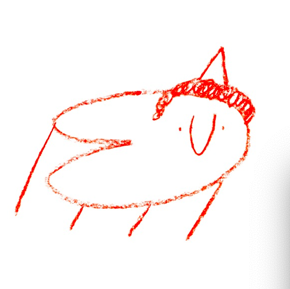
\includegraphics[width = \columnwidth]{./dickbutt.png}
\caption{dickbutt}
\label{fig:"dickbutt"}
\end{figure}
$$
R=\int_{E_0}^0 \frac{dx}{dE}\cdot dE dx
$$


$$
R \propto E_0^{3/2}
$$

$$
x = \frac{c}{c_0}\cdot x_0
$$

## Determining Small Resistance

Measuring small resistances using conventional techniques can be tricky, since oftentimes, the resistance of the circuit itself can be higher than the resistance we are dealing with, which gives us a lot of noise. This can be solved by using lock-in amplifiers.

Using an AC signal, at each frequency, we plot a graph between $V_{DC}$ and $V_{AC}$, and get the slope.

Since $dV_{AC}=RdI_{AC}$m where R is the resistance of the primary circuit, and $dI_{AC}$ is the change in current through the low resistance when the signal generator voltage is changed by $dV_{AC}$. Also, the voltage $V_r$ changes by $dV_r$ where $dV_r=rdI_{AC}$. Therefore, we have:

$$
\frac{dV_{DC}}{dV_{AC}}=\mu \frac{r}{R}
$$

## Determining Mutual Inductance

Changing magnetic fields induces electric fields. Therefore, when a coil of wire is connected to an oscillating voltage, the changing magnetic fields due to it can induce an emf in a coil placed neaby.

Hence, if the current supplied to the primary coil is ,
then the emf induced in the secondary coil is obtained as:

$$
V=-M\frac{dI}{dt}= -2\pi Mft_0 sin(2\pi f t+\frac{\pi}{2})
$$

From above, it is evident that the induced current and the primary current are $90^o$ out of phase. Also, the induced current is directly proportional to the amplitude $I_0$ of the primary current, and it's frequency $f$.

\section{Observations}
\begin{table}[H]
\centering
\resizebox{\columnwidth}{!}{%
\begin{tabular}{|c|c|c|c|c|c|}
\hline
Temperature (in $^oC$) & $V_R$ & $V_C$ & Capacitance (in nF) &  &  \\ \hline
\midrule
21.3 & 3.92 & 1.95 & 0.62 &  &  \\ \hline
50 & 3.95 & 1.95 & 0.63 &  &  \\ \hline
55 & 3.95 & 1.94 & 0.65 &  &  \\ \hline
60 & 3.96 & 1.93 & 0.64 &  &  \\ \hline
65 & 3.97 & 1.91 & 0.67 &  &  \\ \hline
70 & 3.98 & 1.89 & 0.68 &  &  \\ \hline
75 & 4 & 1.85 & 0.71 &  &  \\ \hline
80 & 4.03 & 1.85 & 0.73 &  &  \\ \hline
85 & 4.06 & 1.82 & 0.78 &  &  \\ \hline
90 & 4.10 & 1.75 & 0.82 &  &  \\ \hline
91 & 0.12 & 1.67 & 0.86 &  &  \\ \hline
93 & 4.15 & 1.63 & 0.9 &  &  \\ \hline
95 & 4.12 & 1.57 & 0.93 &  &  \\ \hline
97 & 4.13 & 1.57 & 0.97 &  &  \\ \hline
99 & 4.15 & 1.57 & 1.01 &  &  \\ \hline
100 & 4.19 & 1.57 & 1.03 &  &  \\ \hline
101 & 4.25 & 1.58 & 1.04 &  &  \\ \hline
102 & 4.24 & 1.59 & 1.05 &  &  \\ \hline
103 & 4.24 & 1.6 & 1.06 &  &  \\ \hline
104 & 4.20 & 1.61 & 1.07 &  &  \\ \hline
105 & 4.33 & 1.62 & 1.08 &  &  \\ \hline
106 & 4.25 & 1.6 & 1.1 &  &  \\ \hline
107 & 4.24 & 1.56 & 1.11 &  &  \\ \hline
108 & 4.25 & 1.54 & 1.11 &  &  \\ \hline
109 & 4.26 & 1.54 & 1.1 &  &  \\ \hline
110 & 4.32 & 1.59 & 1.08 &  &  \\ \hline
111 & 4.33 & 1.61 & 1.07 &  &  \\ \hline
112 & 4.37 & 1.62 & 1.06 &  &  \\ \hline
113 & 4.33 & 1.62 & 1.04 &  &  \\ \hline
114 & 4.28 & 1.6 & 1.01 &  &  \\ \hline
115 & 4.20 & 1.58 & 0.98 &  &  \\ \hline
116 & 4.18 & 1.57 & 0.96 &  &  \\ \hline
115 & 4.21 & 1.59 & 0.99 &  &  \\ \hline
114 & 4.20 & 1.6 & 1.01 &  &  \\ \hline
113 & 4.21 & 1.61 & 1.03 &  &  \\ \hline
112 & 4.25 & 1.62 & 1.05 &  &  \\ \hline
111 & 4.23 & 1.63 & 1.07 &  &  \\ \hline
110 & 4.29 & 1.62 & 1.09 &  &  \\ \hline
109 & 4.26 & 11.62 & 1.1 &  &  \\ \hline
108 & 4.24 & 1.58 & 1.11 &  &  \\ \hline
107 & 4.25 & 1.58 & 1.11 &  &  \\ \hline
106 & 4.25 & 1.54 & 1.11 &  &  \\ \hline
105 & 4.21 & 1.37 & 1.12 &  &  \\ \hline
103 & 4.26 & 1.58 & 1.09 &  &  \\ \hline
102 & 4.21 & 1.59 & 1.08 &  &  \\ \hline
101 & 4.25 & 1.6 & 1.07 &  &  \\ \hline
100 & 4.2 & 1.57 & 1.05 &  &  \\ \hline
99 & 4.15 & 1.56 & 1.03 &  &  \\ \hline
97 & 4.2 & 1.54 & 1.00 &  &  \\ \hline
95 & 4.17 & 1.54 & 0.95 &  &  \\ \hline
93 & 4.15 & 1.51 & 0.92 &  &  \\ \hline
91 & 4.07 & 1.5 & 0.88 &  &  \\ \hline
90 & 4.07 & 1.49 & 0.86 &  &  \\ \hline
85 & 4.04 & 1.45 & 0.8 &  &  \\ \hline
75 & 3.58 & 1.43 & 0.73 &  &  \\ \hline
70 & 3.96 & 2.12 & 0.7 &  &  \\ \hline

\end{tabular}%
}
\caption{table1}
\label{tbl:"table1"}
\end{table}
\section{Graphs}
\section{Results}

- The amplification factor was obtained as: $\mu = 1.805 \times 10^3$
- The small resistance was obtained to be: $r =0.031\Omega$
- The mutual inductance of the given coil was obtained as: $M = 120.20 \mu H$

\section{Conclusion}

The functioning of a lock-in amplifier, and its use in extracting signal from noise using phase modulation of the reference signal was studied. These were used in obtaining the resistance of a given small resistance, and the mutual inductance of a given coil.





\clearpage
\end{document}
